\section{What would shorten the queue}
\label{sec:interventions}

\begin{figure}[t]
\centering
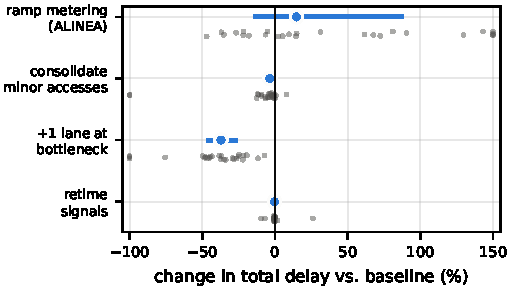
\includegraphics[width=\columnwidth]{figures/interventions.pdf}
\caption{Change in total delay (corridor plus feeder queues) for four
interventions at the CTM's principal bottleneck, over \ItvN\ congested
Monte Carlo direction-runs. Blue: median and interquartile range; grey:
individual runs (clipped at $+150\%$).}
\label{fig:interventions}
\end{figure}

We apply four interventions around the principal bottleneck $b$ in every
congested Monte Carlo run (\ItvN\ direction-runs) and compare total delay
with the same run untreated (Figure~\ref{fig:interventions}).

\paragraph{One more lane over 600\,m at the merge} changes total delay by a
median \ItvLaneMedian\% and helps in \ItvLaneBetter\% of runs. At base parameters
it changes eastbound delay by \ItvLaneBaseEB\%, after which the
next-weakest section becomes the limit. In practice this means extending the frontage road through
the gap, or adding an auxiliary lane on the express side. The model holds
demand fixed, so it omits the extra traffic that new capacity tends to
attract \cite{duranton2011fundamental}.

\paragraph{Ramp metering (ALINEA)} on the four largest feeders within
1.5\,km upstream moves delay rather than removing it: median change
\ItvMetMedian\%, better in \ItvMetBetter\% of runs and worse in
\ItvMetWorse\%. At base parameters eastbound, corridor delay falls from
\ItvBaseEBMain\ to \ItvMetEBMain\,veh\,h while feeder queues grow from
\ItvBaseEBRamp\ to \ItvMetEBRamp. The net gain (\ItvMetBaseEB\%) comes
from avoided capacity drop, and it depends on the drop being large. On an
arterial whose ``ramps'' are residential streets, those waiting vehicles
sit in neighbourhoods.

\paragraph{Consolidating minor accesses} sends residential and service
traffic of each segment to a collector with a single well-designed merge
lane. This removes friction, but it also concentrates the side flow. The
median change is \ItvConMedian\% (better in \ItvConBetter\%, worse in
\ItvConWorse\%).
At base parameters it helps little eastbound (\ItvConBaseEB\%).

\paragraph{Signal retiming} (+0.10 green ratio for the corridor within
1.5\,km upstream and 0.5\,km downstream) barely matters: median
\ItvRetMedian\%. Signals are not where the queue starts, and the green
they gain is taken from cross streets.
